

\tikzset{every picture/.style={line width=0.75pt}} %set default line width to 0.75pt        

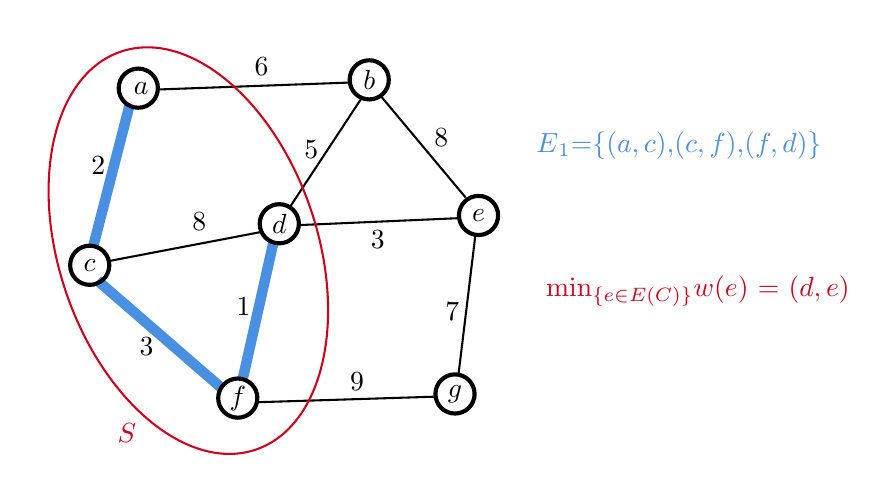
\begin{tikzpicture}[x=0.5pt,y=0.5pt,yscale=-1,xscale=1]
%uncomment if require: \path (0,332); %set diagram left start at 0, and has height of 332

%Straight Lines [id:da823970354045778] 
\draw [color={rgb, 255:red, 0; green, 0; blue, 0 }  ,draw opacity=1 ][line width=0.75]    (269,53) -- (330,126) ;
%Straight Lines [id:da271237396517352] 
\draw [color={rgb, 255:red, 0; green, 0; blue, 0 }  ,draw opacity=1 ][line width=0.75]    (179,274) -- (307,270) ;
%Straight Lines [id:da6657573604931601] 
\draw [color={rgb, 255:red, 74; green, 144; blue, 226 }  ,draw opacity=1 ][line width=3.75]    (64,186) -- (154,264) ;
%Straight Lines [id:da31661075744879486] 
\draw [color={rgb, 255:red, 0; green, 0; blue, 0 }  ,draw opacity=1 ][line width=0.75]    (72,172) -- (182,151) ;
%Straight Lines [id:da9969849240959807] 
\draw [color={rgb, 255:red, 74; green, 144; blue, 226 }  ,draw opacity=1 ][line width=3.75]    (87,60) -- (61,161) ;
%Straight Lines [id:da14506071047898028] 
\draw [color={rgb, 255:red, 0; green, 0; blue, 0 }  ,draw opacity=1 ][line width=0.75]    (107,48) -- (245,43) ;
%Straight Lines [id:da8946288202546534] 
\draw [color={rgb, 255:red, 0; green, 0; blue, 0 }  ,draw opacity=1 ][line width=0.75]    (255,54) -- (203,133) ;
%Straight Lines [id:da15496081521651384] 
\draw [color={rgb, 255:red, 74; green, 144; blue, 226 }  ,draw opacity=1 ][line width=3.75]    (191,159) -- (169,257) ;
%Straight Lines [id:da2163317830574415] 
\draw [color={rgb, 255:red, 0; green, 0; blue, 0 }  ,draw opacity=1 ][line width=0.75]    (337,154) -- (325,253) ;
%Straight Lines [id:da5391246746067021] 
\draw [color={rgb, 255:red, 0; green, 0; blue, 0 }  ,draw opacity=1 ][line width=0.75]    (324,141) -- (209,146) ;
%Shape: Ellipse [id:dp536476356315363] 
\draw  [color={rgb, 255:red, 208; green, 2; blue, 27 }  ,draw opacity=1 ] (41.23,194.4) .. controls (14.29,114.98) and (32.03,37.17) .. (80.86,20.61) .. controls (129.7,4.04) and (191.12,54.99) .. (218.07,134.41) .. controls (245.01,213.83) and (227.27,291.64) .. (178.44,308.21) .. controls (129.6,324.78) and (68.18,273.82) .. (41.23,194.4) -- cycle ;

% Text Node
\draw  [line width=1.5]   (339.38, 139) circle [x radius= 14.15, y radius= 14.15]   ;
\draw (339.38,139) node   [align=left] {$\displaystyle e$};
% Text Node
\draw  [line width=1.5]   (93.48, 47) circle [x radius= 14.15, y radius= 14.15]   ;
\draw (87.98,47) node [anchor=west] [inner sep=0.75pt]   [align=left] {$\displaystyle a$};
% Text Node
\draw  [line width=1.5]   (260.38, 41) circle [x radius= 14.15, y radius= 14.15]   ;
\draw (260.38,41) node   [align=left] {$\displaystyle b$};
% Text Node
\draw  [line width=1.5]   (58.38, 175) circle [x radius= 14.15, y radius= 14.15]   ;
\draw (58.38,175) node   [align=left] {$\displaystyle c$};
% Text Node
\draw  [line width=1.5]   (195.38, 145) circle [x radius= 14.15, y radius= 14.15]   ;
\draw (195.38,145) node   [align=left] {$\displaystyle d$};
% Text Node
\draw  [line width=1.5]   (165.38, 271) circle [x radius= 14.15, y radius= 14.15]   ;
\draw (165.38,271) node   [align=left] {$\displaystyle f$};
% Text Node
\draw  [line width=1.5]   (322.38, 268) circle [x radius= 14.15, y radius= 14.15]   ;
\draw (322.38,268) node   [align=left] {$\displaystyle g$};
% Text Node
\draw (57.24,94.06) node [anchor=north west][inner sep=0.75pt]   [align=left] {$\displaystyle 2$};
% Text Node
\draw (175.24,23.06) node [anchor=north west][inner sep=0.75pt]   [align=left] {$\displaystyle 6$};
% Text Node
\draw (259.24,148.06) node [anchor=north west][inner sep=0.75pt]   [align=left] {$\displaystyle 3$};
% Text Node
\draw (211.24,83.06) node [anchor=north west][inner sep=0.75pt]   [align=left] {$\displaystyle 5$};
% Text Node
\draw (130.24,135.06) node [anchor=north west][inner sep=0.75pt]   [align=left] {$\displaystyle 8$};
% Text Node
\draw (92.24,225.06) node [anchor=north west][inner sep=0.75pt]   [align=left] {$\displaystyle 3$};
% Text Node
\draw (162.24,196.06) node [anchor=north west][inner sep=0.75pt]   [align=left] {$\displaystyle 1$};
% Text Node
\draw (305.24,74.06) node [anchor=north west][inner sep=0.75pt]   [align=left] {$\displaystyle 8$};
% Text Node
\draw (244.24,250.06) node [anchor=north west][inner sep=0.75pt]   [align=left] {$\displaystyle 9$};
% Text Node
\draw (313.24,200) node [anchor=north west][inner sep=0.75pt]   [align=left] {$\displaystyle 7$};
% Text Node
\draw (379,76) node [anchor=north west][inner sep=0.75pt]   [align=left] {$\displaystyle \textcolor[rgb]{0.29,0.56,0.89}{E}\textcolor[rgb]{0.29,0.56,0.89}{_{1}}\textcolor[rgb]{0.29,0.56,0.89}{=}\textcolor[rgb]{0.29,0.56,0.89}{\{}\textcolor[rgb]{0.29,0.56,0.89}{(}\textcolor[rgb]{0.29,0.56,0.89}{a,c}\textcolor[rgb]{0.29,0.56,0.89}{)}\textcolor[rgb]{0.29,0.56,0.89}{,}\textcolor[rgb]{0.29,0.56,0.89}{(}\textcolor[rgb]{0.29,0.56,0.89}{c,f}\textcolor[rgb]{0.29,0.56,0.89}{)}\textcolor[rgb]{0.29,0.56,0.89}{,}\textcolor[rgb]{0.29,0.56,0.89}{(}\textcolor[rgb]{0.29,0.56,0.89}{f,d}\textcolor[rgb]{0.29,0.56,0.89}{)}\textcolor[rgb]{0.29,0.56,0.89}{\}}$};
% Text Node
\draw (76.24,287.06) node [anchor=north west][inner sep=0.75pt]   [align=left] {$\displaystyle \textcolor[rgb]{0.82,0.01,0.11}{S}$};
% Text Node
\draw (386,180) node [anchor=north west][inner sep=0.75pt]   [align=left] {$\displaystyle \textcolor[rgb]{0.82,0.01,0.11}{\min}\textcolor[rgb]{0.82,0.01,0.11}{_{\{e\in E( C)\}}}\textcolor[rgb]{0.82,0.01,0.11}{w}\textcolor[rgb]{0.82,0.01,0.11}{(}\textcolor[rgb]{0.82,0.01,0.11}{e}\textcolor[rgb]{0.82,0.01,0.11}{)}\textcolor[rgb]{0.82,0.01,0.11}{\ =\ }\textcolor[rgb]{0.82,0.01,0.11}{(}\textcolor[rgb]{0.82,0.01,0.11}{d,e}\textcolor[rgb]{0.82,0.01,0.11}{)}$};


\end{tikzpicture}

